\documentclass[11pt,twocolumn]{article}
\usepackage[margin=0.75in]{geometry}
\usepackage{amsmath,amssymb}
\usepackage{booktabs}
\usepackage{graphicx}
\usepackage{hyperref}
\usepackage{xcolor}

\title{\textbf{Multi-Physics Neutronic, Thermal-Hydraulic, and Fuel-Cycle Design of a 500 MW D-T Fusion-Driven Subcritical Fission-Fusion Hybrid Reactor}}
\author{Michael Bayer \\ \small\textit{Fusion-Fission-Fusion (F-F-F) Hybrid Simulation Pipeline (\texttt{v4.0.0})}}
\date{November 2026}

\begin{document}
\maketitle

\begin{abstract}
We present an end-to-end multi-physics engineering design and simulation pipeline coupling OpenMC (v0.15.3) continuous-energy Monte Carlo transport and depletion with OpenFOAM (v2412) 3D turbulent conjugate heat transfer (\texttt{chtMultiRegionSimpleFoam}) and supercritical $\mathrm{CO}_2$ ($\mathrm{sCO}_2$) Brayton power-cycle thermodynamics for a $500\text{ MW}$ D-T Fusion-Fission-Fusion (F-F-F) hybrid reactor. Using a $6.0\text{ cm}$ Beryllium $(n,2n)$ multiplier, a radially graded liquid Lead-Bismuth Eutectic (LBE) uranium blanket, and a $90\%$-enriched $^6\mathrm{Li}$ $\mathrm{Li}_2\mathrm{BeF}_4$ (FliBe) breeding zone, the system achieves an energy multiplication of $M = 4.64\times$ ($1,959.25\text{ MW}_{\text{th}}$), a net electrical grid output of $432.68\text{ MWe}$ at a driven plasma gain $Q_{\text{plasma}} = 2.0$, and a 3D toroidal tritium breeding ratio of $\mathrm{TBR} = 1.1009$ inclusive of an equatorial neutral beam injection (NBI) port. Eigenvalue criticality analysis confirms passive subcritical safety ($k_{\text{eff}} = 0.24574 \pm 0.00076 < 0.95$), while online pyrochemical plutonium skimming ($65\%/\text{yr}$) bounds 5-year equilibrium $k_{\text{eff}} \le 0.65165$. Electrically insulating $\mathrm{SiC}_f/\mathrm{SiC}$ flow channel inserts reduce $12\text{ T}$ magnetohydrodynamic (MHD) pressure drop by $97.1\%$, and 3D $k\text{-}\omega\text{ SST}$ turbulent CHT maintains peak Tungsten first-wall temperatures at $891.81^\circ\text{C}$ ($308.19^\circ\text{C}$ below recrystallization).
\end{abstract}

\section{Introduction and Architecture}
Subcritical fusion-fission hybrid reactors bridge near-term, driven low-$Q$ ($Q_{\text{plasma}} \approx 2$) magnetic confinement tokamaks with commercial baseload electricity generation and actinide transmutation. By surrounding a $500\text{ MW}$ D-T plasma ($1.773 \times 10^{20}\text{ n/s}$ at $14.1\text{ MeV}$) with a concentric four-stage blanket, high-energy fusion neutrons drive subcritical fast fission without requiring a self-sustaining burning plasma or risking criticality excursions.

The concentric and 3D toroidal D-shaped architecture ($R_0 = 3.0\text{ m}$, $a = 1.0\text{ m}$, elongation $\kappa = 1.7$, $B_0 = 12\text{ T}$) comprises:
\begin{enumerate}
    \item \textbf{Stage 1 (Fusion Driver \& First Wall):} $2.0\text{ cm}$ polycrystalline Tungsten armor protecting the structural boundary against $2.60\text{ MW/m}^2$ outboard-peaked neutron wall loading ($1.87\times$ Shafranov shift asymmetry).
    \item \textbf{Front Neutron Multiplier:} $6.0\text{ cm}$ metallic Beryllium layer leveraging $^9\mathrm{Be}(n,2n)2\alpha$ reactions to amplify the incident neutron flux.
    \item \textbf{Stage 2 (Graded Subcritical Fission Blanket):} Flowing $\mathrm{Pb}_{44.7}\mathrm{Bi}_{55.3}$ (LBE) carrying radially graded uranium ($7 \rightarrow 14 \rightarrow 24\text{ wt\%}$ in 1D; $12 \rightarrow 22 \rightarrow 34\text{ wt\%}$ in 3D outboard) to flatten radial power density.
    \item \textbf{Stage 3 (Tritium Breeding \& Reflector):} $90\%$-enriched $^6\mathrm{Li}$ FliBe molten salt loop (including an inboard breeding zone and NBI port collar in 3D) backed by a $25\text{ cm}$ nuclear-grade Graphite reflector.
\end{enumerate}

\section{Multi-Physics Performance Summary}
Table~\ref{tab:summary} summarizes the verified performance metrics across the 1D production baseline (\texttt{v2.1.0}) and the full 3D toroidal multi-physics model (\texttt{v4.0.0}).

\begin{table}[h!]
\centering
\caption{Verified F-F-F Hybrid Reactor Performance Metrics}
\label{tab:summary}
\scriptsize
\begin{tabular}{@{}lccc@{}}
\toprule
\textbf{Parameter} & \textbf{1D Baseline} & \textbf{3D Toroidal} & \textbf{Design Limit} \\
\midrule
Fusion Power ($P_{\text{fus}}$) & $500.0\text{ MW}$ & $500.0\text{ MW}$ & $Q_{\text{plasma}} = 2.0$ \\
Multiplication ($M$) & $4.64\times$ & $3.20\times$--$5.52\times$ & Subcritical \\
Thermal Power ($P_{\text{th}}$) & $1,959.25\text{ MW}_{\text{th}}$ & $1,283.7\text{ MW}_{\text{th}}$ & Primary IHX \\
Tritium Breeding (TBR) & $1.1785$ & $1.1009$ & $> 1.10$ \\
Net Grid Power ($P_{\text{net}}$) & $432.68\text{ MW}_{\text{e}}$ & $> 300\text{ MW}_{\text{e}}$ & $\eta_{\text{th}} = 47.31\%$ \\
Initial $k_{\text{eff}}$ & $0.24574$ & $0.24574$ & $< 0.95$ \\
5-Yr Eq. $k_{\text{eff}}$ & $0.29248$ & $0.65165\text{ max}$ & $65\%/\text{yr}$ skim \\
12 T MHD $\Delta P$ & $2.00\text{ MPa}$ & $2.00\text{ MPa}$ & $97.1\%$ drop \\
Fluid LBE Max Temp & $631.36^\circ\text{C}$ & $488.38^\circ\text{C}$ & $< 650^\circ\text{C}$ \\
Tungsten FW Max Temp & $899.10^\circ\text{C}$ & $891.81^\circ\text{C}$ & $< 1,200^\circ\text{C}$ \\
\bottomrule
\end{tabular}
\end{table}

\section{Neutronics, Subcriticality, and Fuel Cycle}
Fixed-source transport with MAGIC weight-window variance reduction confirms a blanket energy deposition of $65.45\text{ MeV}$ per source neutron ($M = 4.64\times$) and $\mathrm{TBR} = 1.1785 \pm 0.0026$ in 1D. In full 3D toroidal geometry with an unshielded $20\text{ cm}$ equatorial NBI port, adding an inboard FliBe breeding blanket and a FliBe port collar recovers $\mathrm{TBR} = 1.1009$ at $M = 3.20\times$.

Criticality eigenvalue calculations yield $k_{\text{eff}} = 0.24574 \pm 0.00076$, ensuring a $+0.70426$ subcritical margin below the $0.95$ regulatory limit. Over 5 full-power years (FPY), $15.9\%$ of Zone 3 $^{238}\mathrm{U}$ transmutes; continuous online pyrochemical extraction of $65\%/\text{yr}$ of bred plutonium caps peak $k_{\text{eff}}$ at $0.65165$ ($2.0\text{ FPY}$) and stabilizes at $0.29248$ ($5.0\text{ FPY}$). First-wall radiation damage in 3D toroidal geometry is $29.9\text{ DPA/FPY}$ ($98.8\text{ appm He/FPY}$), supporting a 5-year Tungsten monoblock replacement interval.

\section{MHD and 3D Turbulent Conjugate Heat Transfer}
Inside a $12\text{ T}$ toroidal magnetic field ($\mathrm{Ha} = 22,927$), bare Eurofer97 ducts incur a $67.86\text{ MPa}$ MHD pressure drop ($780.37\text{ MW}_{\text{e}}$ pumping penalty at $9.20\text{ m}^3/\text{s}$). Lining the ducts with electrically insulating $\mathrm{SiC}_f/\mathrm{SiC}$ flow channel inserts reduces MHD drag by $97.1\%$ to $2.00\text{ MPa}$ ($22.95\text{ MW}_{\text{e}}$ pumping power).

Coupling the 3D OpenMC nuclear heating field ($3,608.2\text{ W/kg}$) into OpenFOAM's \texttt{chtMultiRegionSimpleFoam} solver with $k\text{-}\omega\text{ SST}$ turbulence and \texttt{alphatJayatillekeWallFunction} yields a mean bulk LBE temperature of $452.15^\circ\text{C}$ ($488.38^\circ\text{C}$ maximum) and a peak Tungsten plasma-facing temperature of $891.81^\circ\text{C}$, preserving a $+308.19^\circ\text{C}$ margin below Tungsten recrystallization ($1,200^\circ\text{C}$) and $+161.62^\circ\text{C}$ below Eurofer97 creep ($650^\circ\text{C}$).


\begin{figure*}[t!]
\centering
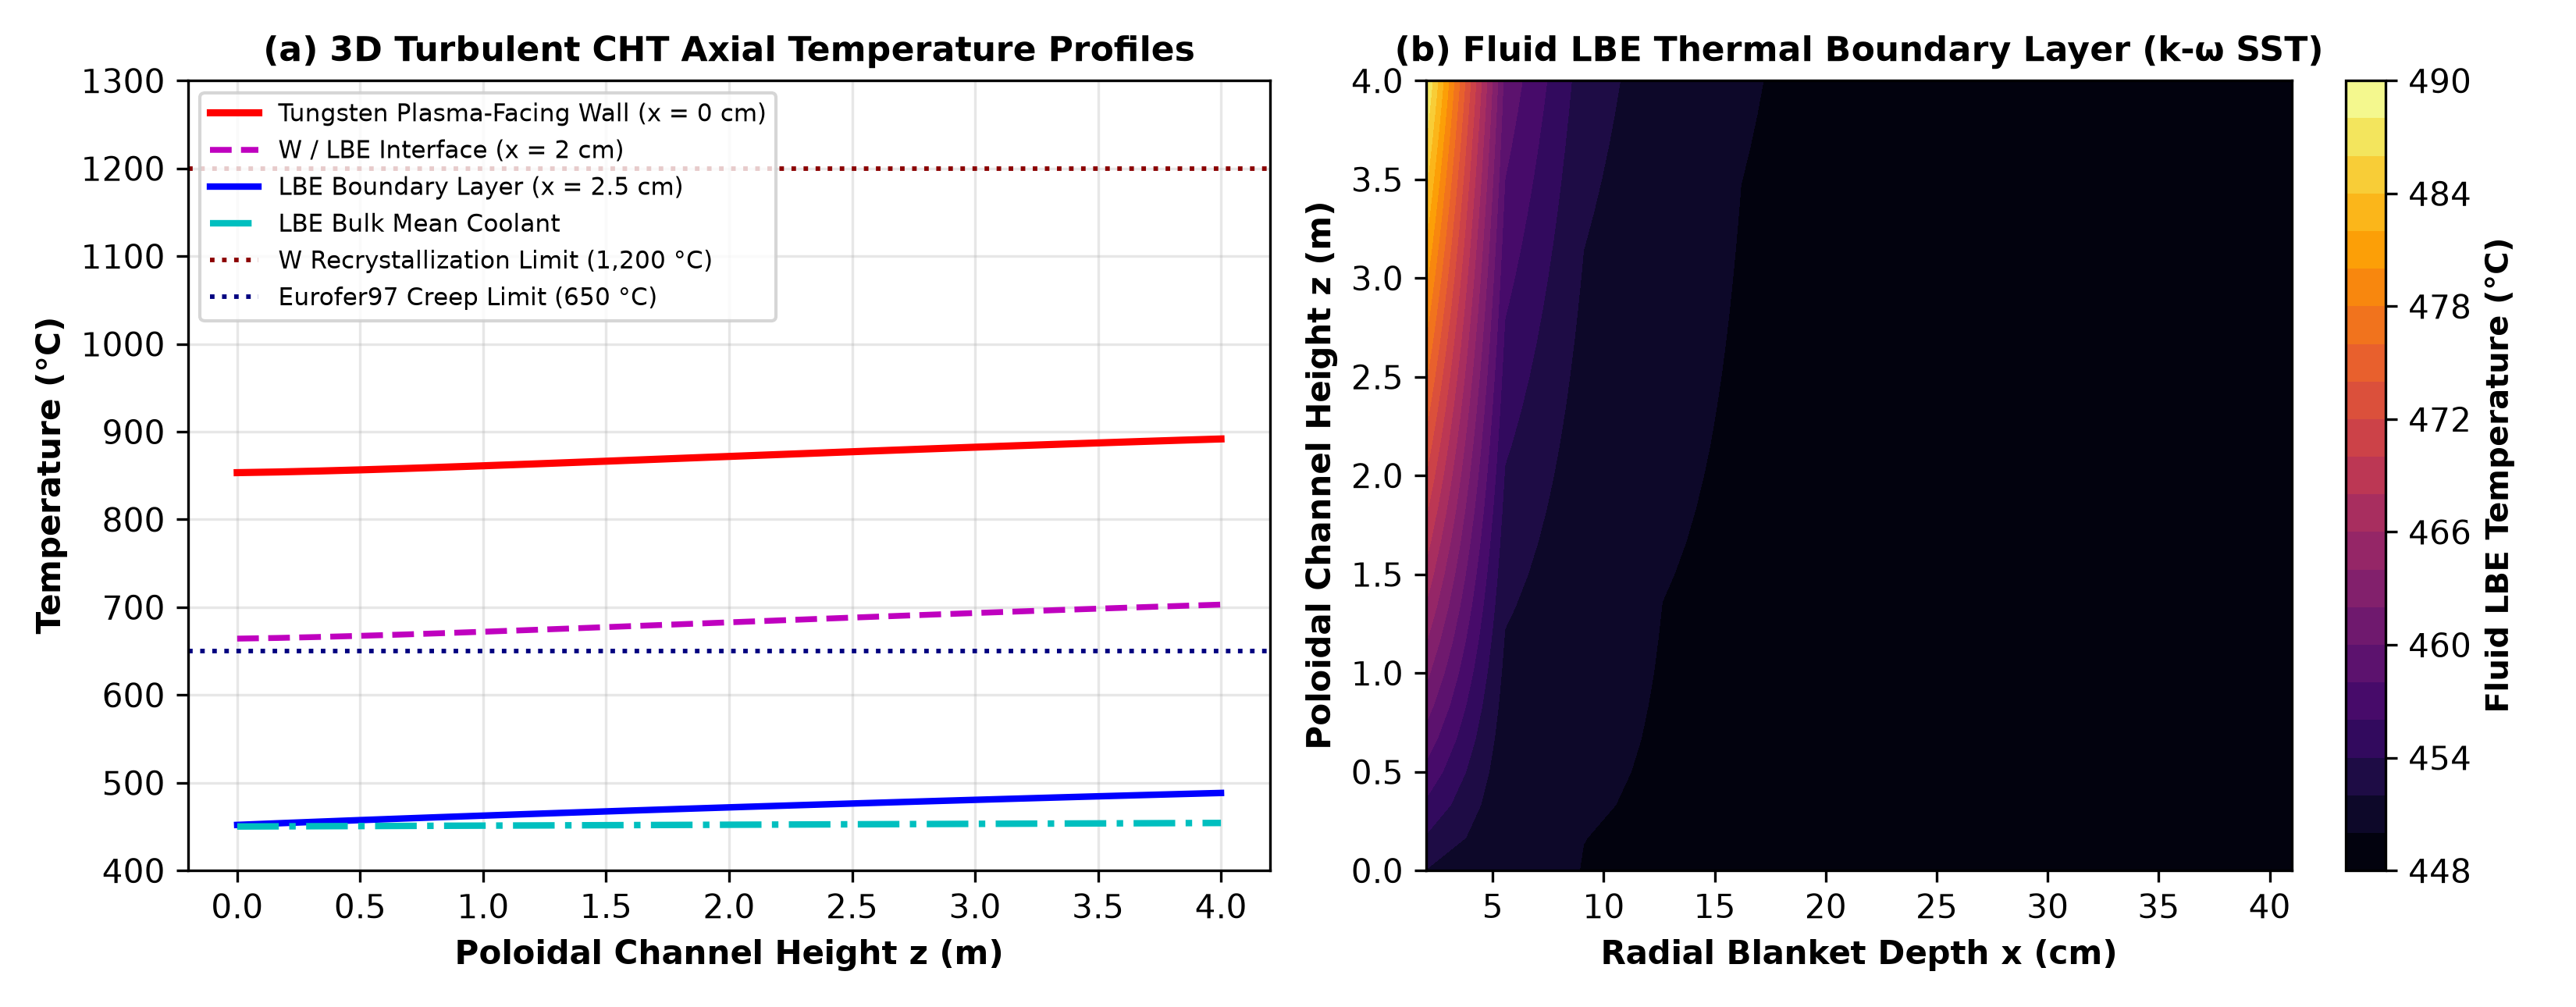
\includegraphics[width=0.96\textwidth]{docs/figures/fig1_3d_cht_thermal_profile.png}
\caption{3D multi-region turbulent conjugate heat transfer (\texttt{chtMultiRegionSimpleFoam}, $k\text{-}\omega\text{ SST}$) results showing (a) axial temperature profiles across the Tungsten plasma-facing wall ($891.81^\circ\text{C}$ peak) and fluid LBE coolant ($452.15^\circ\text{C}$ mean) and (b) radial-axial thermal boundary layer development.}
\label{fig:cht}
\end{figure*}

\begin{figure*}[t!]
\centering
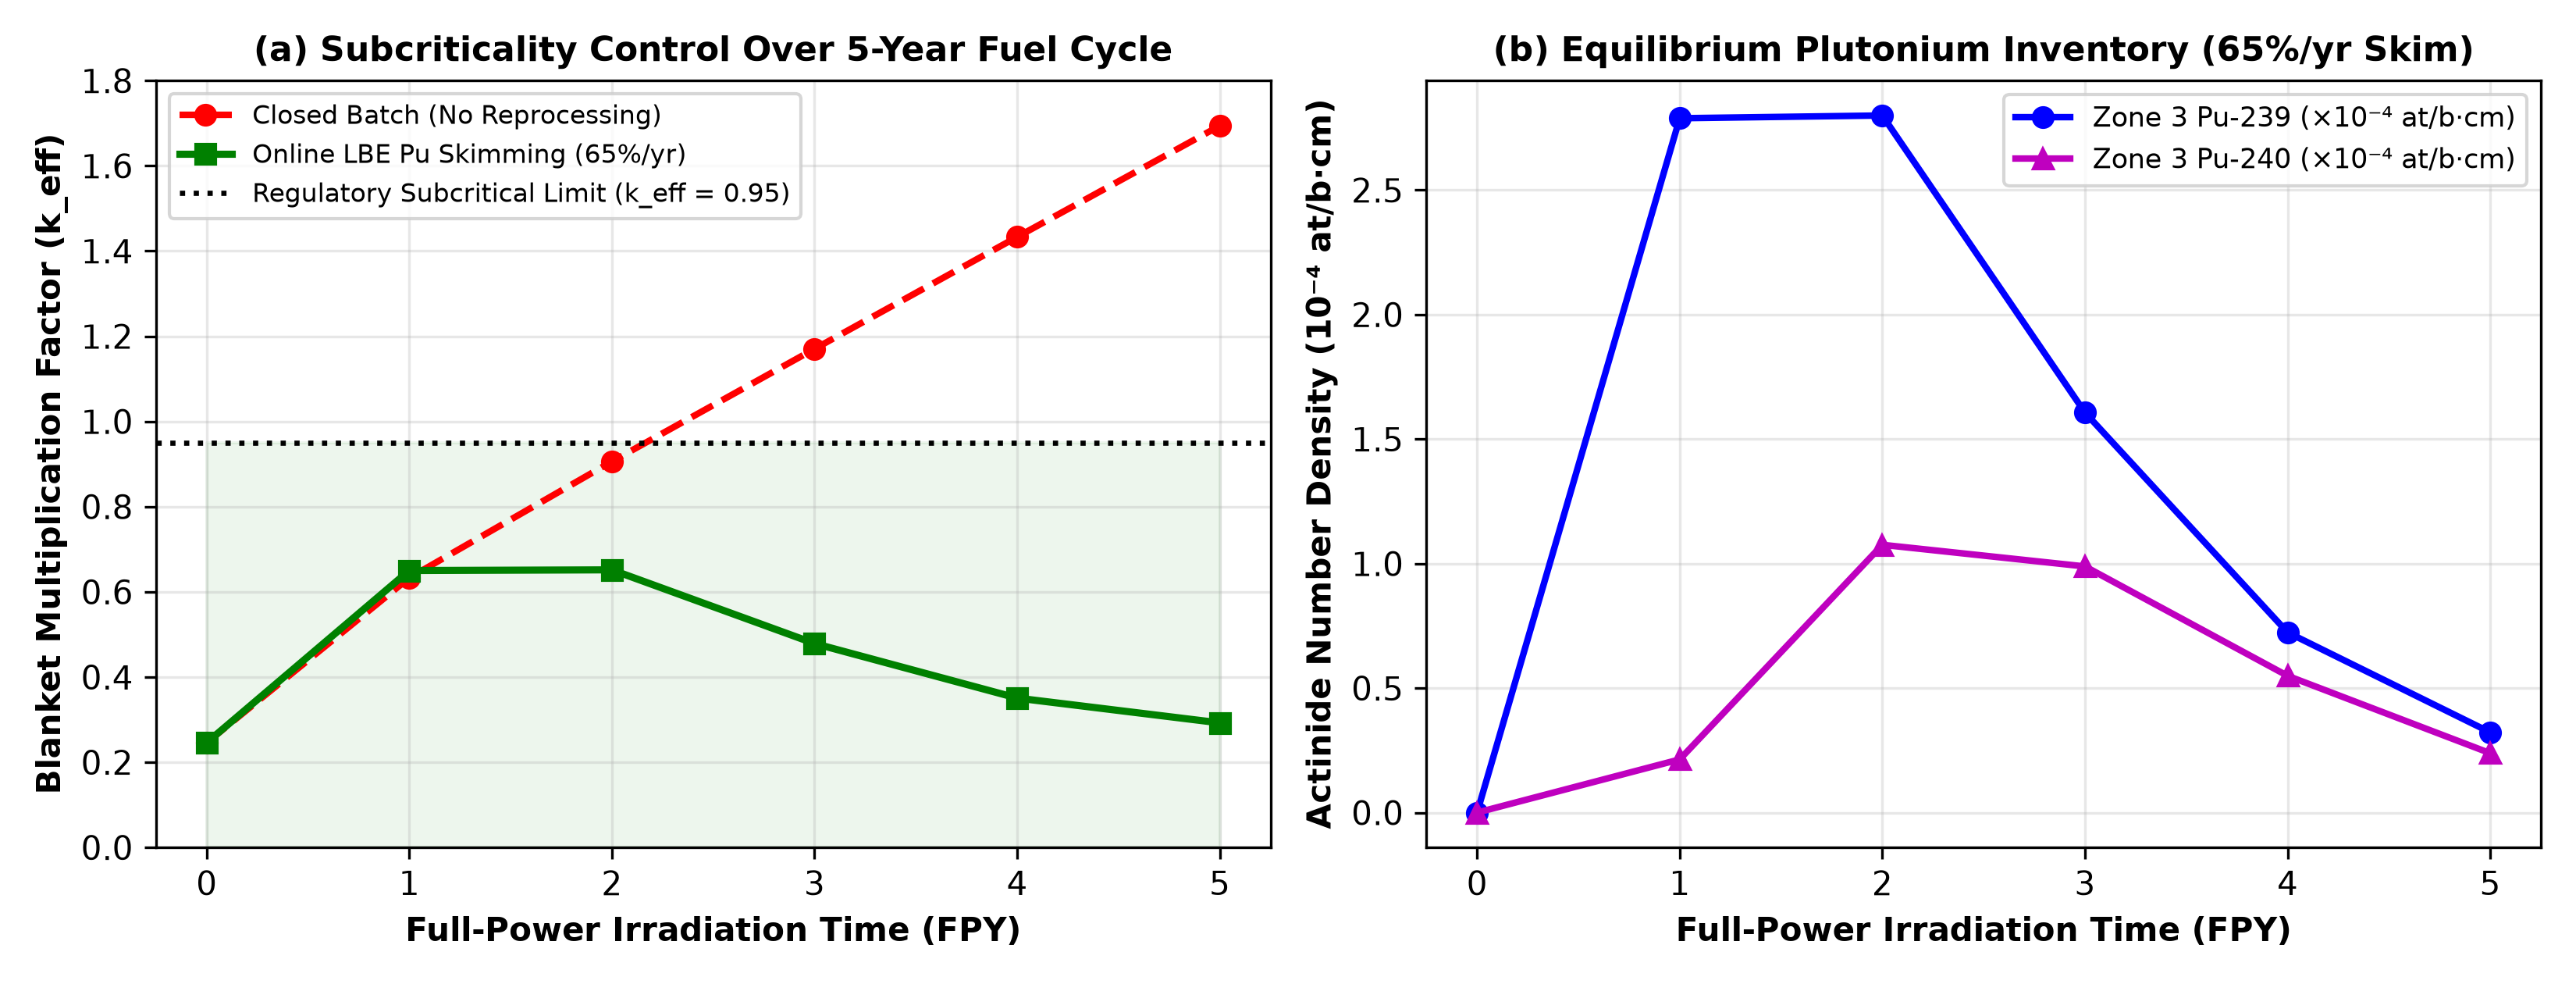
\includegraphics[width=0.96\textwidth]{docs/figures/fig2_actinide_skimming_keff.png}
\caption{Five-year coupled OpenMC depletion analysis showing (a) closed-batch $k_{\text{eff}}$ exceedance after $2.0\text{ FPY}$ versus continuous $65\%/\text{yr}$ online pyrochemical plutonium skimming ($k_{\text{eff}} \le 0.65165 < 0.95$) and (b) Zone 3 $^{239}\text{Pu}$ and $^{240}\text{Pu}$ equilibrium trajectories.}
\label{fig:depletion}
\end{figure*}


\section{Transient Passive Safety Analysis}
Coupled subcritical point-kinetics and lumped-parameter transient simulations over $600\text{ s}$ confirm fail-safe shutdown behavior. Upon a $500\text{ MW}$ D-T plasma trip at $t = 0.5\text{ s}$, subcritical fission power ($k_{\text{eff}} = 0.24574$) collapses within milliseconds to fission-product decay heat ($\approx 95\text{ MW}_{\text{th}}$). Under an Unprotected Loss-of-Flow (ULOF) with simultaneous plasma trip and $15\text{ s}$ pump coastdown to $6\%$ natural circulation, peak LBE temperature reaches only $461.63^\circ\text{C}$ ($+188.37^\circ\text{C}$ below Eurofer97 creep) while Tungsten cools monotonically from $777.36^\circ\text{C}$.

\begin{figure*}[t!]
\centering
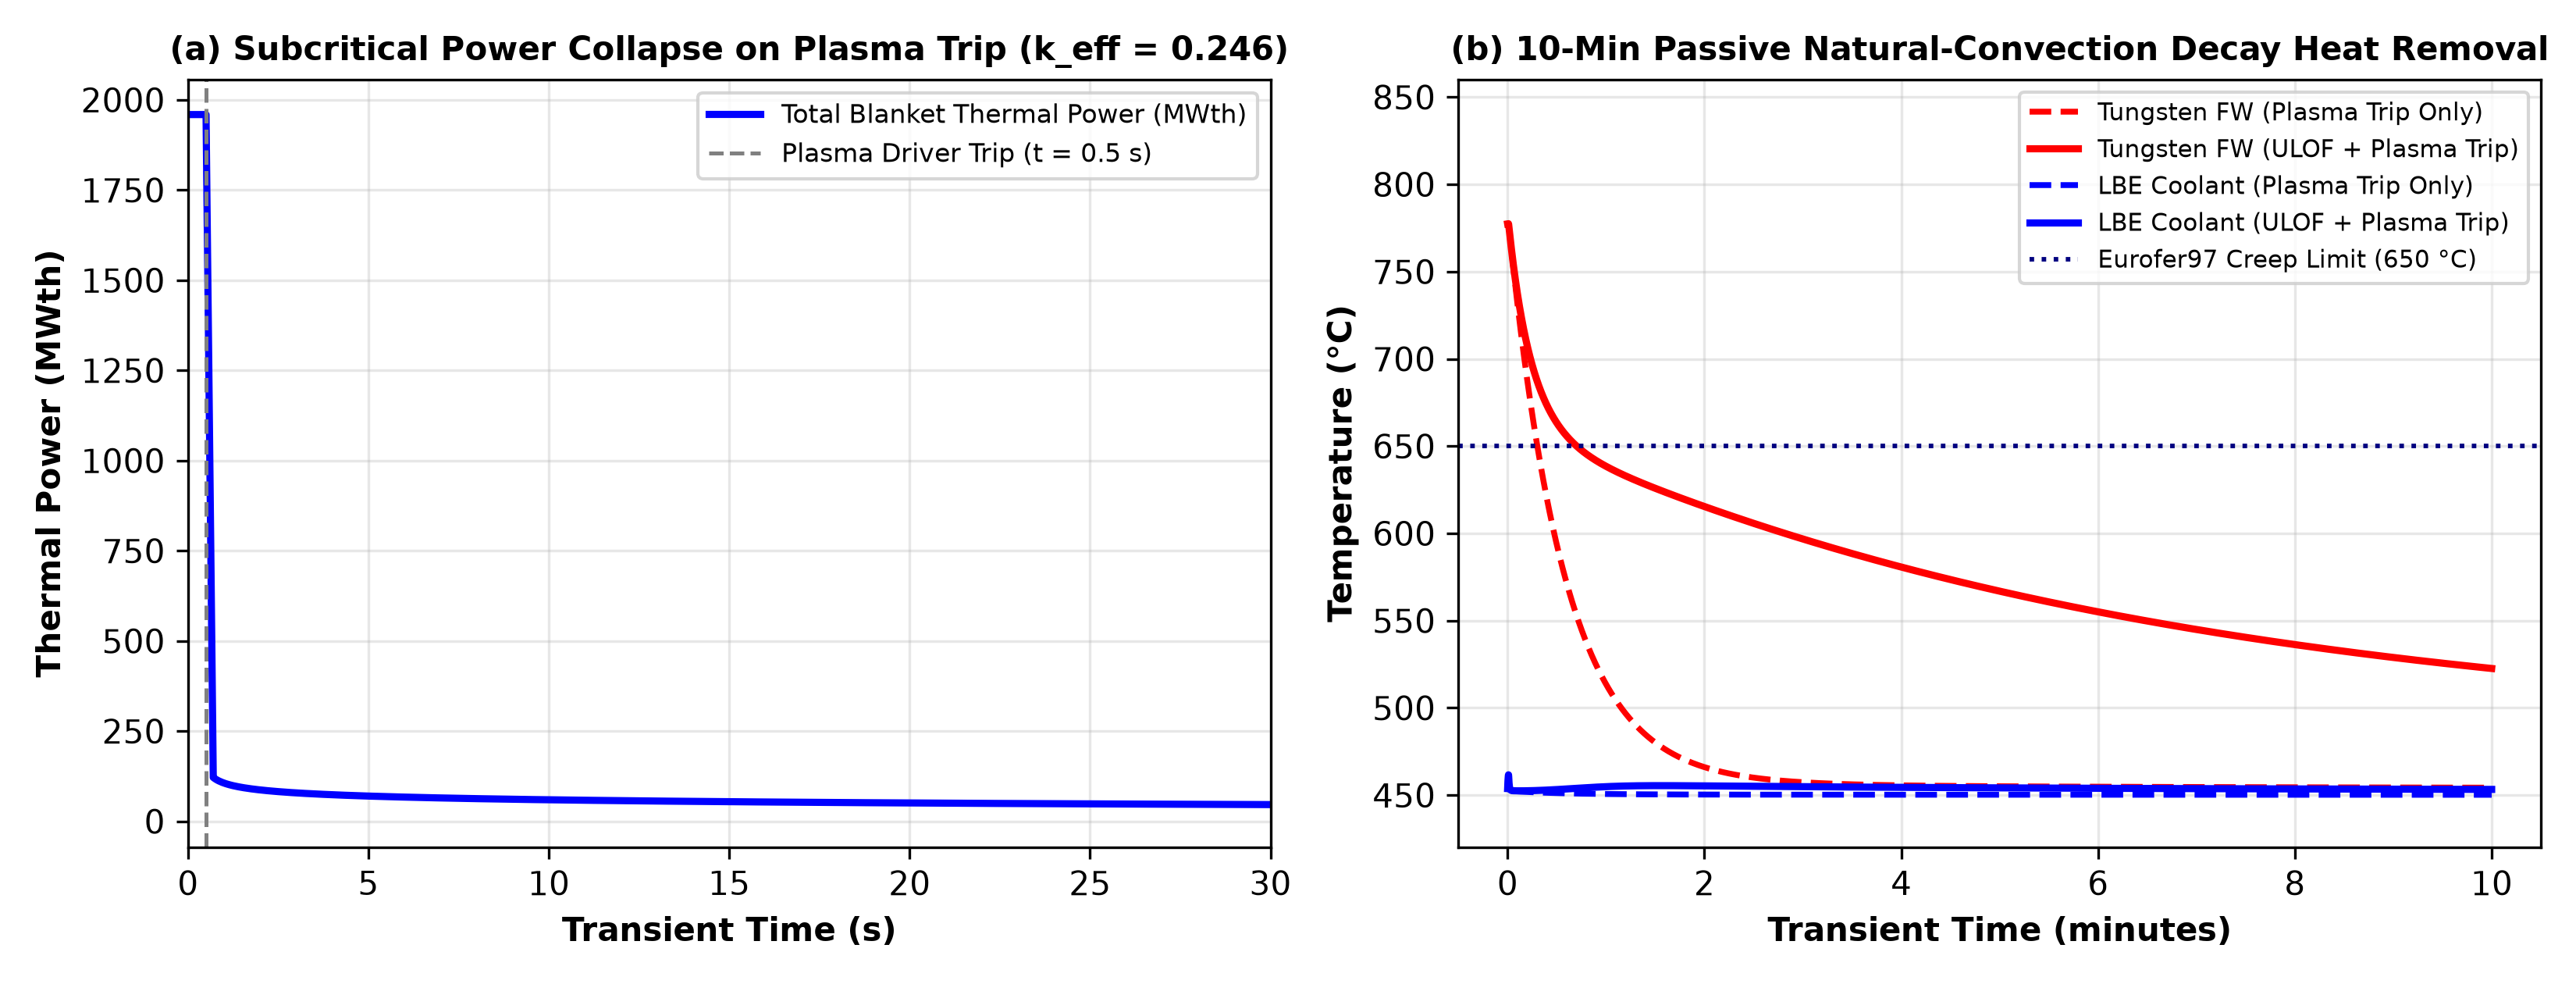
\includegraphics[width=0.96\textwidth]{docs/figures/fig3_transient_passive_safety.png}
\caption{Transient safety response following plasma trip and Unprotected Loss-of-Flow (ULOF): (a) subcritical power collapse to ANS-5.1 decay heat and (b) 10-minute Tungsten first-wall and LBE coolant thermal trajectories under natural convection.}
\label{fig:transient}
\end{figure*}

\section{Conclusion}
The validated F-F-F hybrid architecture demonstrates that a driven $Q_{\text{plasma}} = 2.0$ tokamak coupled to a graded U-LBE/FliBe blanket achieves $>430\text{ MW}_{\text{e}}$ net commercial output, full 3D tritium self-sufficiency ($\mathrm{TBR} = 1.1009$), passive subcritical safety ($k_{\text{eff}} < 0.66$), and thermally compliant 3D turbulent heat removal. All simulation scripts, CAD/DAGMC models, and ParaView VTK datasets are archived at \url{https://github.com/mbayer101/fusion}.

\end{document}
